\chapter{Uncertainty Quantification in a Real-World Clinical Task: Deprescribing} \label{chapter:deprescribing}

\section{Introduction}
The aim of this thesis is to assess uncertainty quantification (UQ) and, in doing so, evaluate the Bayesian diagnostic reasoning capabilities of large language models (LLMs). A fundamental requirement for Bayesian diagnostic reasoning is a comprehensive understanding and quantification of clinical uncertainty. Clinical judgment frequently demands both qualitative and quantitative interpretations of uncertainty \cite{feinsteinClinicalJudgmentRevisited1994a}. For instance, the LLM must be able to quantify the uncertainty associated with a differential list of diagnoses to determine the most useful diagnostic test to run next, similar to how a physician would reason about a patient during diagnostic wayfinding. However, in a similar scenario, the relative risks associated with a particular patient situation may convince a physician to choose a less sensitive diagnostic test with lower risk. For instance, a patient being evaluated for a colorectal cancer may be recommended to get a colonoscopy, which is the gold-standard diagnostic test for detecting cancers and precancerous polyps. However, a prior traumatic medical experience may contribute to their anxiety around sedation and complications, leading a physician to perform a fecal immunochemical (FIT) test, despite the quantitative risk suggesting a colonoscopy. Therefore, while the quantitative interpretation of uncertainty may be relevant in determining the "ideal" decision making process, qualitative elements influence decision making. These sometimes competing priorities contribute to the art and science of medicine and require clinical gestalt. An LLM that attempts to align with current clinical practice must handle both these qualitative and quantitative interpretations of uncertainty. In this work, we tackle the former through an inherently qualitative uncertainty quantification task: the process of recommendation deprescribing in older adults (i.e. $\geq$ 65 years old). 

Deprescribing is defined as the systematic process of identifying and discontinuing drugs, called potentially inappropriate medications (PIMs), whose present or potential harms outweigh benefits provided to the patient within the context of their individual care goals and quality of life \citep{hohlPolypharmacyAdverseDrugrelated2001a, scottReducingInappropriatePolypharmacy2015}. This process is primarily conducted in patients that are at-risk for drug-related negative outcomes: those with polypharmacy regimes. Widely defined as the regular use of at least five medications, polypharmacy is common in older adults and at-risk populations\citep{halli-tierneyPolypharmacyEvaluatingRisks2019}. In fact, approximately 30\% of patients aged 65 years or older have polypharmacy\citep{scottReducingInappropriatePolypharmacy2015}, and nearly half of older emergency department (ED) patients are discharged with one or more new medications\cite{skainsGeriatricEmergencyMedication2024}. Although necessary and beneficial for some patients, polypharmacy can increase risk of negative consequences for patients, including emergency department (ED) visits, adverse drug events (ADEs), falls, disability, and inappropriate medication use\cite{halli-tierneyPolypharmacyEvaluatingRisks2019}.

Deprescribing tools, such as the Screening Tool of Older People's Prescriptions (STOPP)\citep{omahonySTOPPSTARTCriteria2023} and Beers\citep{bythe2023americangeriatricssocietybeerscriteriarupdateexpertpanelAmericanGeriatricsSociety2023} criteria, have been developed to help providers assess and identify PIMs based on a patient's medication list\citep{candeiasPotentiallyInappropriateMedications2021,kaufmannInappropriatePrescribingSystematic2014}. These explicit assessments are criterion-based with clear standards, but are often impractical to implement in time-constrained clinical settings, such as the emergency department\citep{leeChallengesOpportunitiesCreating2022}. Attempts to digitize these criteria into electronic clinical decision support have raised difficulties, typically requiring a labor-intensive coding process and unstructured information from patient records to contextualize certain criteria\citep{anrysSTOPPSTARTVersion2016b, scottUsingEMRenabledComputerized2018}. Large language models (LLMs) have been shown to interpret complex clinical situations and offer recommendations, from differential diagnoses to care management, leading to growing interest in their application in the medical field\citep{clusmannFutureLandscapeLarge2023, gilsonHowDoesChatGPT2023, kungPerformanceChatGPTUSMLE2023, savageDiagnosticReasoningPrompts2024}. Moreover, they have been shown to extract medication-related data such as medication name, dosage, and frequency, necessary for application of deprescribing criteria\citep{goelLLMsAccelerateAnnotation2023}. Lastly, LLMs are excellent in-context learners, requiring very little labeled data to make predictions\citep{agrawal-etal-2022-large} reducing the annotation burden for time-constrained EM physicians while improving the use of unstructured patient records to contextualize patient medication lists. However, the majority of clinical reasoning evaluations on LLMs have been conducted using standardized exams (USMLE) or online case reports\citep{savageDiagnosticReasoningPrompts2024, savageLargeLanguageModel2024}. Both of these exam types are multiple choice and require clinical gestalt and reasoning to make decisions under  qualitative clinical uncertainty. In some cases, patient considerations need to be taken into account. In most, explicit quantification of benefits and risks is unnecessary, and instead relative risks are weighed against one another, in combination with guidelines and rules of thumb. However, LLMs ability to perform this form of qualitative reasoning over physician-generated text (such as clinical notes) remains unclear.  

In this chapter, we propose to evaluate the performance of an end-to-end LLM-based pipeline in recommending deprescribing options for older adult ED patients at discharge based on explicit deprescribing criteria, such as the Beers and STOPP criteria. This work will help address gaps in electronic deprescribing by using an LLM to contextualize recommendations within individual patient records and reduce manual development in clinical decision support (CDS) tools. More relevant to the uncertainty quantification goals of this thesis, we also apply selective prediction methods to evaluate an LLM's ability to abstain based on its internal model of clinical uncertainty and defer decision making to a human reviewer. By investigating these methods, we aim to better understand how well an LLM's internal model of clinical uncertainty aligns with that of physicians and whether it can provide calibrated, reliable support in real-world scenarios. Together with our work in quantitative interpretations of uncertainty by the LLM in Chapters \ref{chapter:race-bayes} and \ref{chapter:bn-reasoning}, we aim to deepen our understanding of clinical uncertainty and its impact on the effectiveness of LLM-based CDS systems.

\section{Methods}

In this section, we describe our evaluation framework that incorporates a two-step LLM pipeline, comparison with medical students as junior annotators, discrepancy adjudication by senior annotators (board-certified EM physicians), and the introduction of selective prediction methods in a human-in-the-loop decision making framework. The final component functions to both evaluate the LLM's internal model of qualitative clinical uncertainty, as well as how this model may be used to function within a shared clinical decision making system in a real world clinical setting. 

\subsection{Patient Cohort}

Our cohort consists of all older adults ($\geq$ 65 yo.) with polypharmacy ($\geq$ 5 active outpatient medications) presenting to the Yale New Haven-Health Emergency Department between January-March 2022 totaling 10,977 patients across 15,161 encounters. We selected a random convenience sample of 100 unique patients with 941 total medications. Given the nature of the criteria, all outpatient medications were filtered to only include oral medications, leading to 712 total oral medications and a median of 6 medications per patient (Figure \ref{fig:aim1-demographics}). From our initial study cohort of 100 patients, 5 patients each were set aside for both prompt engineering and inter-rater reliability (IRR) between junior annotators. Following our iterative prompt engineering approach described below, our final cohort consisted of 92 patients with 626 medications. Our sample size was guided by budget constraints and a power analysis of deprescribing rates from an informal screening study (target sample size: 560 medications; population deprescribing incidence: 10\%\citep{garfinkelWarPolypharmacyNew2007}; screening study incidence: 5.88\%\citep{SAEM24Abstracts2024}; power: 0.95; alpha: 0.05). 

\begin{figure}[!htbp]
	\centering
	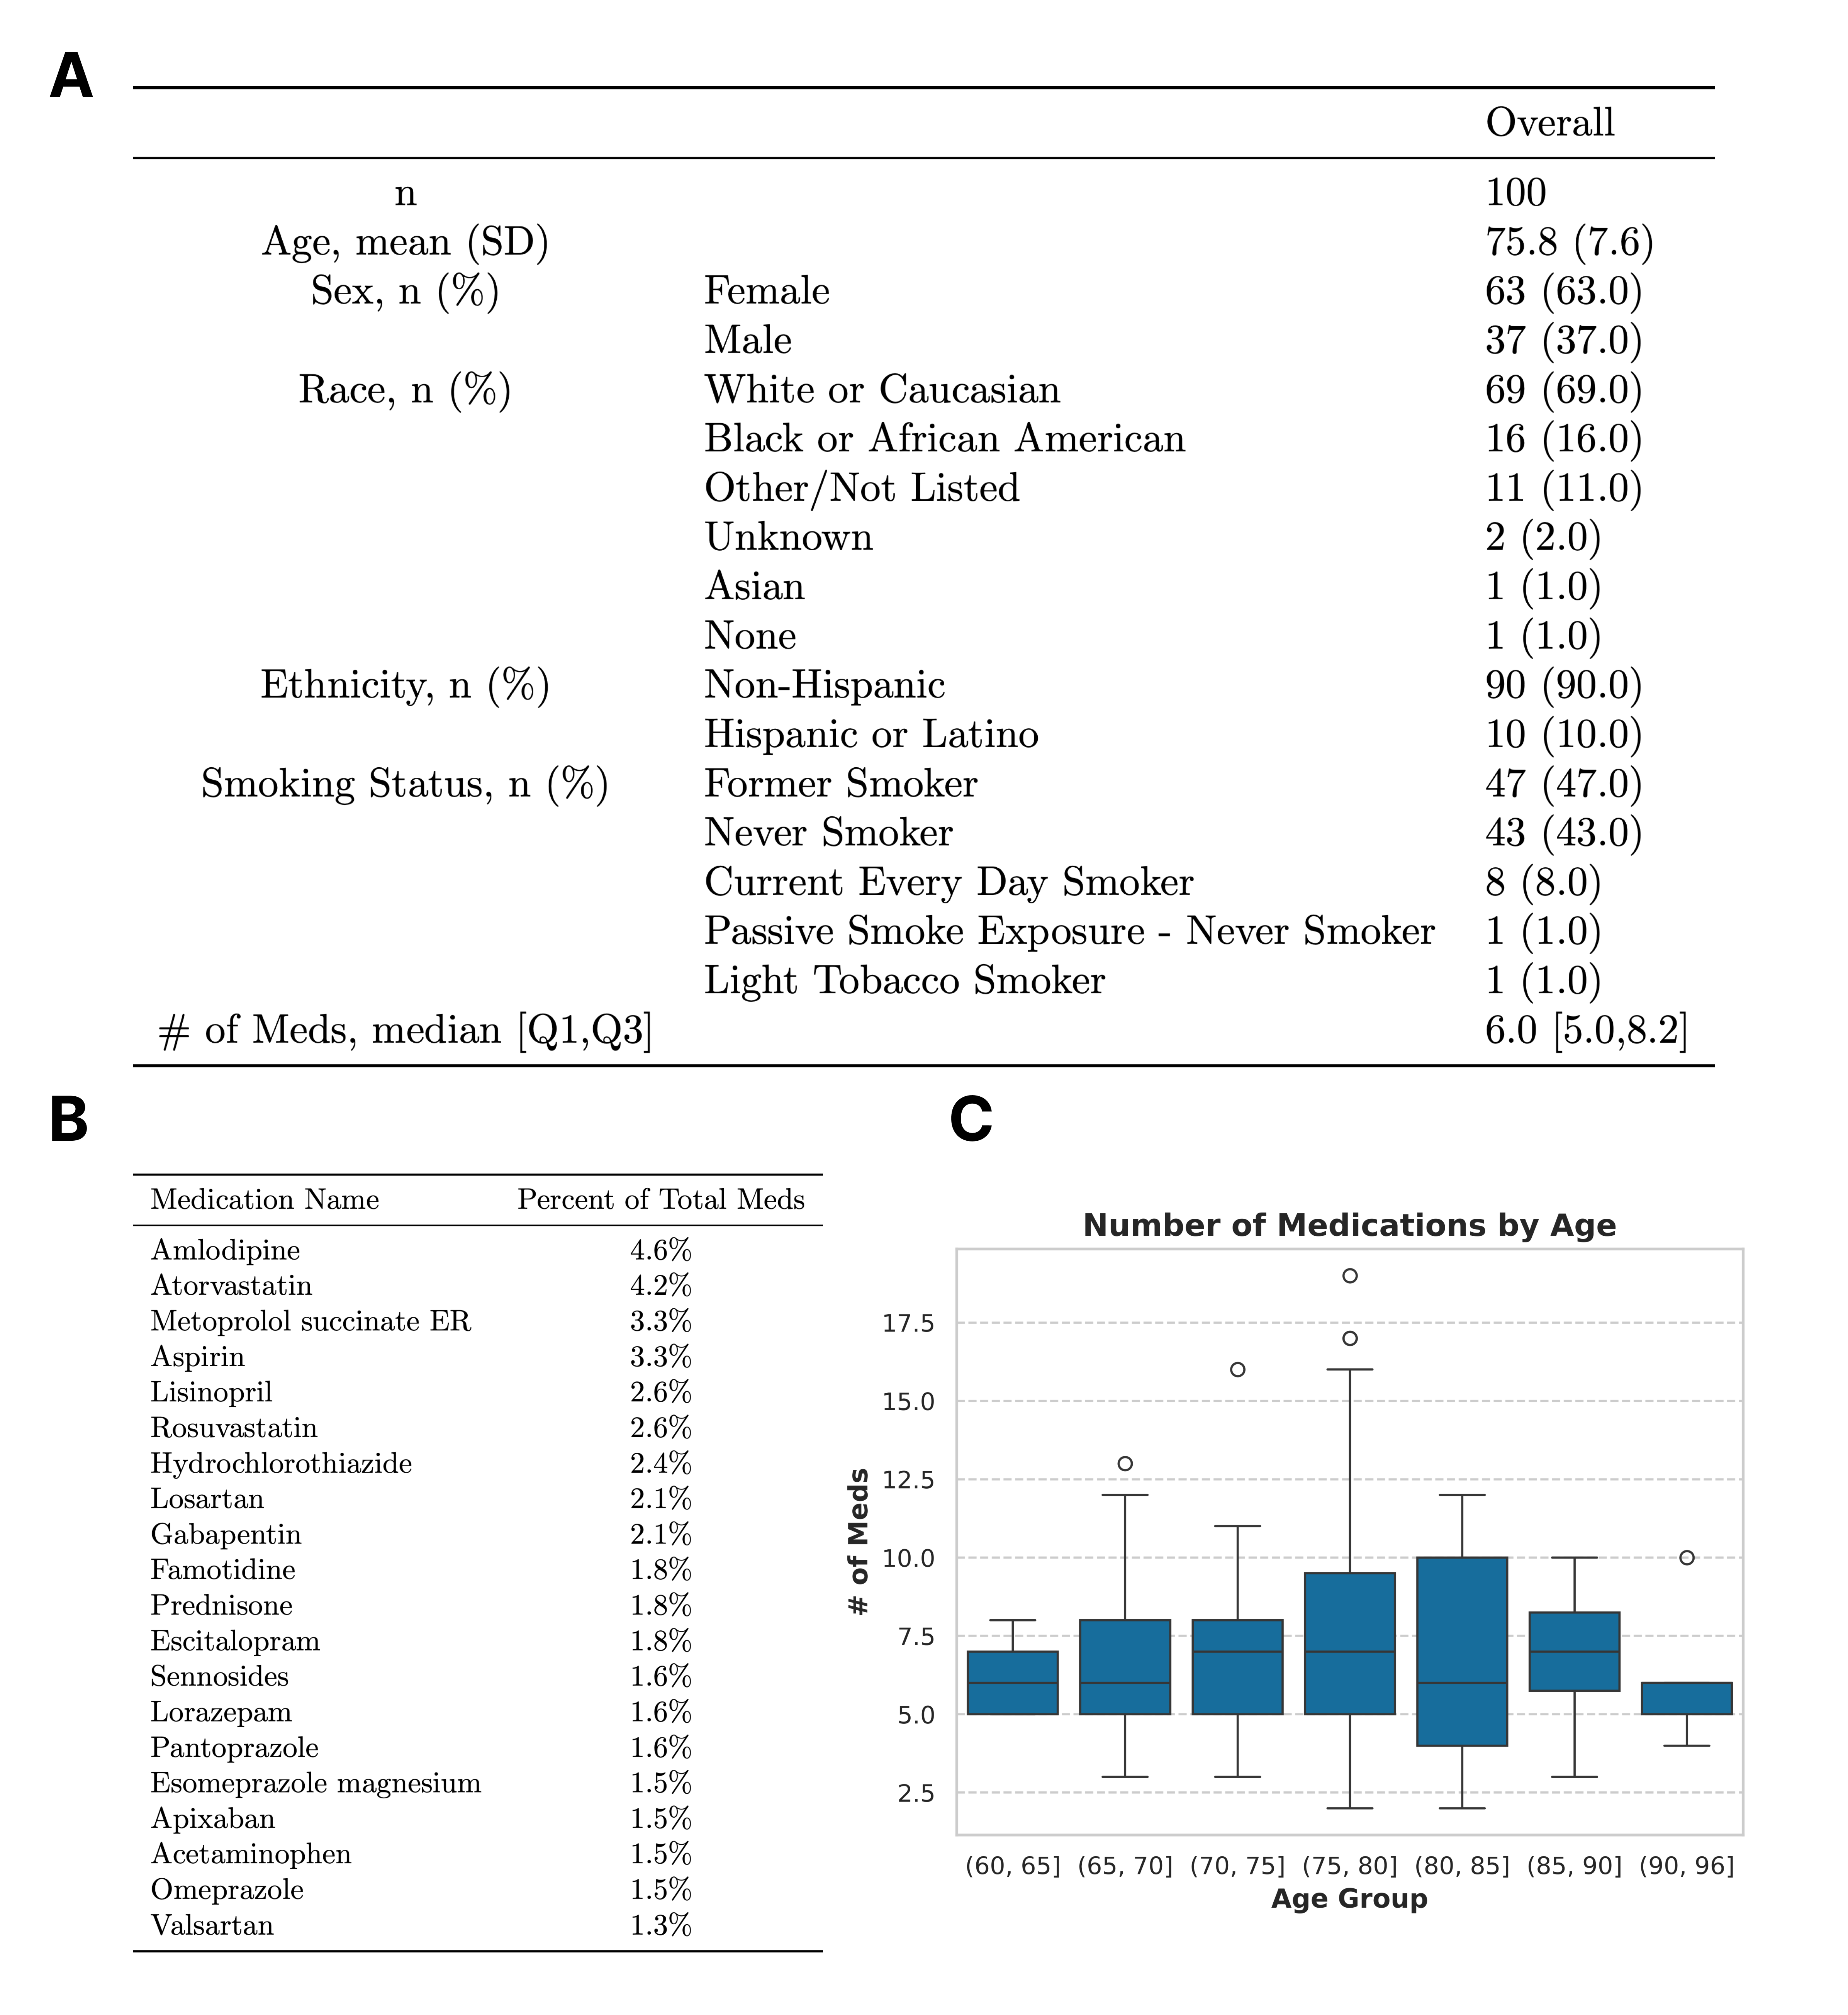
\includegraphics[width=1\textwidth] {figures/aim1/combined_fig.png}
	\caption{Basic demographics of the polypharmacy deprescribing cohort evaluated. (A) Demographic overview of the 100 patients included in the evaluation. (B) The top 20 most commonly prescribed medications, represented as a percentage of the total medication set. (C) Distribution of medications across different age groups.} \label{fig:aim1-demographics}
\end{figure}


\subsection{Consensus-Based High-Yield Criteria Evaluation}

In our screening study\citep{SAEM24Abstracts2024}, one of the main causes of discrepancies between physicians and LLMs arose from ambiguous inclusion/exclusion conditions in deprescribing criteria. For example, criteria like \emph{"Statins for primary cardiovascular prevention in persons aged $\geq$85 with established frailty with expected life expectancy likely less than 3 years."} include elements—such as \emph{"established frailty"} and \emph{"expected life expectancy"}—that are challenging to quantify and therefore difficult to implement computationally. To address these issues and identify only those criteria that are high-yield, we conducted a rigorous, consensus-based evaluation of deprescribing criteria from three recommendation lists: STOPP\citep{omahonySTOPPSTARTCriteria2023}, Beers\citep{bythe2023americangeriatricssocietybeerscriteriarupdateexpertpanelAmericanGeriatricsSociety2023}, and GEMS-Rx\citep{skainsGeriatricEmergencyMedication2024}. 

We evaluated 180 recommendations across two key dimensions: Clinical Applicability and EHR Computability. Within the 5 clinical applicability questions, we focused on Clinical Risk to filter our criteria. High-yield criteria were defined as those posing significant clinical risk to the patient and being identifiable within the EHR. These dimensions were chosen to ensure that a GPT-enabled clinical decision support (CDS) tool prioritizes meaningful recommendations—reducing alert fatigue from unnecessary alerts—and has access to high-quality EHR data, enabling accurate, actionable deprescribing recommendations. The consensus panel consisted of 6 board-certified physicians (in Emergency Medicine, Internal Medicine, Clinical Informatics, and Internal Medicine-Pediatrics) and 1 ED pharmacist at YNHH. Each member of the group individually reviewed each of the criteria and rated them on a 5-point Likert scale. The average results of the consensus study are presented and used to filter to a final set of high-yield criteria. 

\subsection{Deprescribing Recommendations by GPT-4o}

\begin{figure}[!htbp]
	\centering
	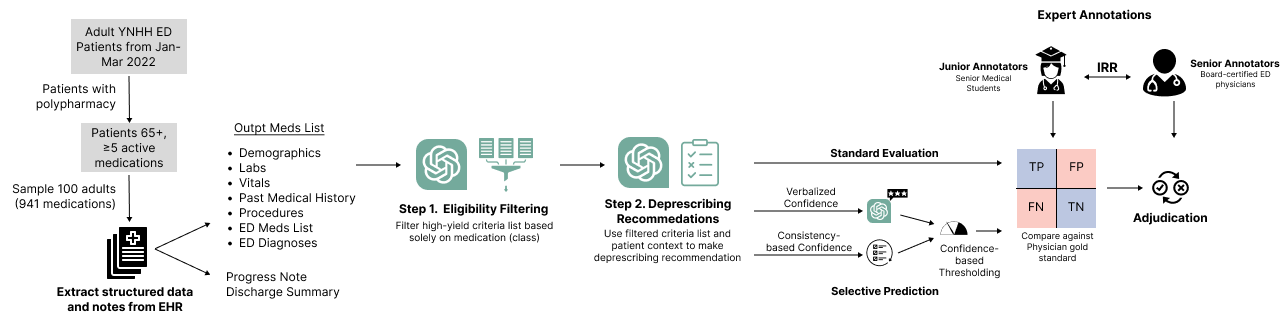
\includegraphics[width=1\textwidth] {figures/aim1/methods_overview.png}
	\caption{Overview of the evaluation pipeline, consisting of a two-step GPT process, performance comparison with junior annotators (medical students), and final adjudication by senior annotators (board-certified physicians). The full prompts for Step 1 and Step 2 are included in the Supplementary Figures (Figure~\ref{fig:aim1-step1-prompt} and \ref{fig:aim1-step2-prompt}).} \label{fig:aim1-overview}
\end{figure}


Our initial testing revealed that providing the LLM with the full set of criteria and medications led to simple reasoning errors. The large number of criteria, combined with the simultaneous processing of the complete patient medication list, resulted in inaccuracies in applying individual criteria to specific medications. To address this, we implemented a two-step pipeline where the criteria were first filtered and then recommendations were generated, applying this process independently to each medication, as shown in Figure \ref{fig:aim1-overview}. In step 1, GPT-4o is prompted to filter the full list of high-yield criteria solely based on the patient's medication list, ignoring inclusion/exclusion conditions. This both reduces confusion due to large input context sizes\citep{liuLostMiddleHow2024} and ensures that extraneous context does not  distract the LLM\citep{shiLargeLanguageModels2023}. In step 2, GPT-4o is prompted to use its previously filtered criteria list, along with structured (e.g. demographics, lab values, vitals, and PMH) and unstructured (most recent progress note and discharge summary) information, to determine if the patient satisfies any deprescribing criteria and therefore should be recommended for deprescribing. 

To ensure optimal performance, we engineered prompts in an iterative fashion\citep{safranekAutomatedHEARTScore2024}, using one patient at a time from the held-out set of 5 patients. After each evaluation, prompts were adjusted to correct any systematic errors (e.g., instances where no relevant criteria in step 1 led to non-criteria-based deprescribing recommendations in step 2) by the LLM. After processing three patients without identifying additional errors during manual inspection, we concluded that further adjustments were unnecessary. Consequently, the final two patients in the held-out set were included in the final cohort evaluation (n=92 patients, 626 medications). Aside from the consistency-based method, described below, all LLM calls are performed with fully limited randomness (temperature=0, set seed). 

\subsection{Selective Prediction}

In addition to assessing performance relative to medical students, we examine whether the LLMs' apparently well-calibrated confidence in question-answering tasks, such as the USMLE, extends to real-world clinical recommendation tasks\cite{singhalLargeLanguageModels2023}. To do so, we collected GPT-4o's decision confidence for both steps using two validated confidence elicitation methods: chain-of-thought verbalized confidence and self-random sampling with average-confidence aggregation, referred to as consistency-based confidence\cite{xiongCanLLMsExpress2023}. In verbalized confidence, we ask the LLM to explicitly estimate its confidence for each step following its decision. For the consistency-based approach, we query the LLM multiple times (N=5) with high temperature (T=0.8) and use a verbalized confidence-weighted confidence estimate. In a human-in-the-loop decision making system, the LLM's confidence would be used to determine if the model should abstain due to low certainty regarding its own decision. In practice, this case would be considered too difficult for the LLM and forwarded to an expert reviewer. This human-in-the-loop decision making pipeline is known as selective prediction and has been commonly found to improve performance in non-text-based applications\cite{leibigLeveragingUncertaintyInformation2017, chuaTacklingPredictionUncertainty2023}. We evaluate both selective prediction methods using risk-coverage curves\cite{geifmanSelectiveClassificationDeep2017, el-yanivFoundationsNoisefreeSelective2010}, substituting coverage for LLM deferring fraction, and conduct a more in-depth analysis of the method that proves to be more effective.

\subsection{Comparison and Adjudication with Clinical Experts}

\begin{table}
\centering
\caption{Definitions of GPT-4o error modes inspired by framework from \citet{lievinCanLargeLanguage2024} relevant to deprescribing recommendations.}
\begin{tabular}{p{0.2\textwidth}p{0.38\textwidth}p{0.38\textwidth}}\toprule
Error Mode & Definition & Example \\ \midrule
Reading comprehension & Includes misunderstanding of order of text, such as when a medication is dependent on another medication in a specific arrangement. Also includes omission of information provided to the model, such as missing a relevant category explicitly stated in the recommendations. & GPT failed to recognize acetaminophen by name from the list of STOPP criteria in a patient at risk for malnutrition/liver disease. \\
Recall of knowledge & Includes failure to recognize classes of medications or other medical facts necessary to perform the task. & GPT correctly recognized amlodipine was a calcium channel blocker but failed to recognize it was more broadly an antihypertensive. \\
Incorrect reasoning step & Faulty reasoning, such as inappropriate assumptions or leads of logic unsupported by the clinical data. & GPT recommended discontinuing warfarin in a patient with a therapeutically elevated INR after assuming that this elevated INR was due to a bleeding disorder. \\
Not enough information & Inappropriate application of missing data leading to potentially unreliable conclusions, such as assuming abnormality of a missing laboratory study. & GPT recommended discontinuing a QT prolonging antidepressant based on the possibility of QT prolongation without any ECG data or history of abnormal QT interval. \\\bottomrule
\end{tabular}%
\label{tab:aim1-error-modes}
\end{table}

In this study, we utilized a multi-stage human review and adjudication process to assess model performance. To simulate a scenario where a pharmacy technician or trainee would screen for potential PIMs, two senior medical students (M4) evaluated all medications in the test cohort, with discrepancies between the students (junior annotators) and the LLM adjudicated by two board-certified ED physicians (senior annotators). This two-stage process allowed us to both simulate the real conditions of having a technician or trainee perform the screening task while still utilizing a more senior physician in the adjudication stage to define the gold standard response. For each medication, a medical student would determine (1) if there exists a relevant high-yield criteria based on the medication list, and (2) whether the medication should be recommended for deprescribing. Of the 712 total oral medications, 75 (from 5 patients) were evaluated by both medical students to measure inter-rater reliability (IRR). We then computed discrepancies between medical students and the LLM and provided them to the ED physicians to determine who was correct and in cases where the LLM was incorrect, why this was the case. We leveraged a prior evaluation framework\citep{lievinCanLargeLanguage2024} to determine LLM error modes. We classified each error as one of four relevant error modes: incorrect reading comprehension, incorrect recall of knowledge, incorrect reasoning step, and not enough information, as described in Table \ref{tab:aim1-error-modes}. We measured the IRR between the two senior ED physicians to ensure that coding practices were standardized prior to adjudication on the full set of GPT-medical student discrepancies. 

\section{Results}

In this section, we present the results of our consensus-based evaluation, which aimed to identify high-yield criteria, assess GPT-4o's performance relative to junior annotators (medical students), and analyze the adjudication process, including attribution of correct judgments and characterization of GPT's error modes. Furthermore, we evaluate the LLM's ability to estimate its qualitative uncertainty and explore how this capability impacts the implementation of selective prediction methods within a human-in-the-loop decision-making framework. 

\subsection{Consensus-Based High-Yield Criteria Evaluation}

The average scores, separated by deprescribing criteria list, for each of 5 questions of clinical applicability and 4 questions of EHR computability are shown in Figure \ref{fig:aim1-suvey-results}. We classified criteria with a clinical risk (Q1) rating greater than 3 and an average EHR computability rating (Q6-Q9) greater than 3. However, this led to a high number of potentially high-yield criteria (n=162 criteria). To further narrow the criteria, we then selected the top 50\% criteria arriving at 81 total criteria across all three deprescribing lists. A plot of our selected criteria as a function of EHR computability and patient risk is shown in Supplementary Figure \ref{fig:aim1-consensus-avg-ratings}. On average, STOPP criteria both had the lowest clinical risk and EHR computability ratings and Beers, the highest. This was primarily attributed to panelists' concerns that the information required by STOPP criteria was not readily accessible within the EHR and would necessitate additional data at the point of care. Additionally, GEMS-Rx had the lowest ED feasibility rating (2.75) compared to STOPP (2.93) and Beers (2.91). 

\begin{figure}[!htbp]
	\centering
	\includegraphics[width=1\textwidth] {figures/aim1/survey_results.png}
	\caption{Average distribution of results on 5-point Likert scale from consensus study by expert panel (n=7) split by three criteria lists: Beers, GEMS-Rx, and STOPP.} \label{fig:aim1-suvey-results}
\end{figure}

\subsection{Deprescribing Recommendations by GPT-4o}


Consistent with our screening study, the medical student inter-rater reliability (IRR) in both steps was low (Cohen's k: step 1–0.741 , step 2–0.082) across 75 medications. This led to an exploration of their performance compared to GPT-4o. As shown in Figure \ref{fig:aim1-confmat}, approximately half the medications (~50.3\%) did not have relevant high-yield deprescribing criteria. However, there were a number of discrepancies that needed to be adjudicated. Of these, 52 (8.30\%) were less clinically significant as, despite the discrepancy on criteria eligibility, both the medical student and the GPT-4o model ultimately decided deprescribing was not necessary. In contrast, 64 medications (10.2\% of the total) were cases where either GPT-4o or the medical student disagreed on deprescribing, potentially impacting medication management. Notably, a major source of discrepancy was the significantly higher likelihood of the LLM to recommend deprescribing (11.6\%) compared to the medical students (1.91\%).

\begin{wrapfigure}{l}{0.65\textwidth}
	\centering
	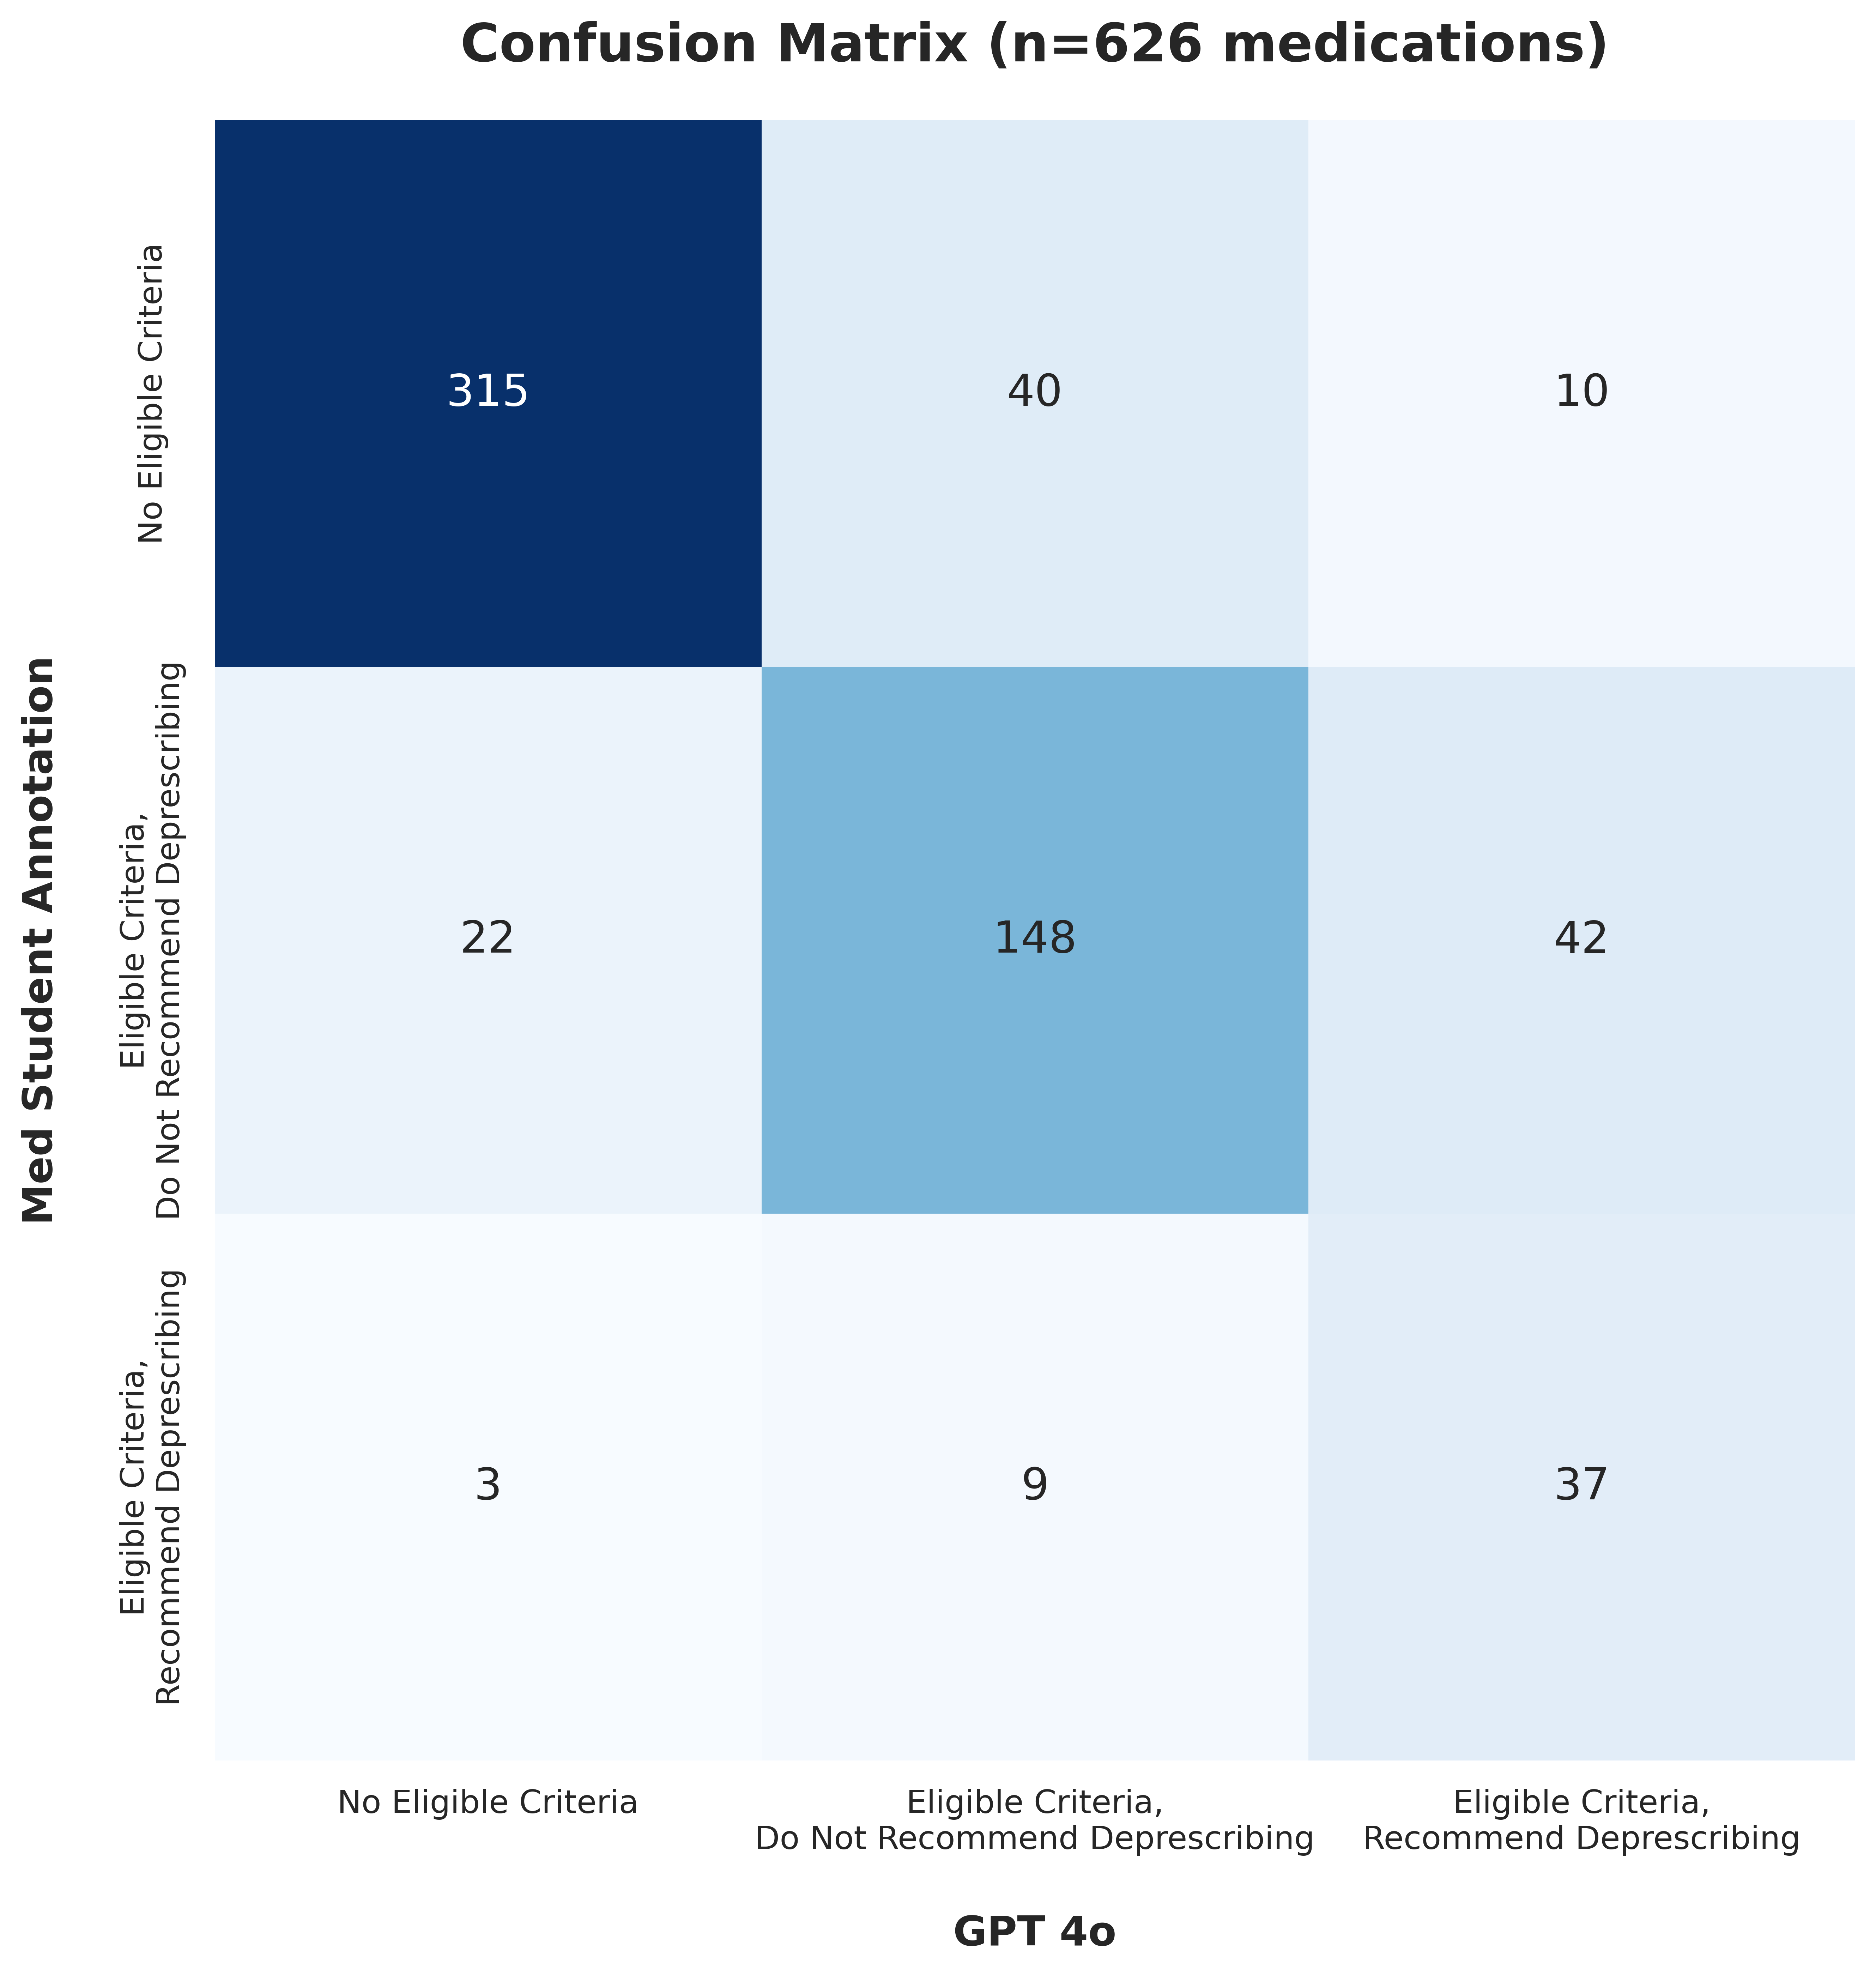
\includegraphics[width=0.6\textwidth] {figures/aim1/medstudent_gpt_confmat.png}
	\caption{Joint confusion matrix across both steps showing alignment and discrepancies between GPT-4o model and medical students. } \label{fig:aim1-confmat}
\end{wrapfigure}


Two senior annotators (board-certified EM physicians) adjudicated the 126 discrepancies between GPT 4o and the junior annotators following codebook standardization and verification of IRR (Cohen's k: Eligibility–0.795, Deprescribing–0.745). We found that across all discrepancies, GPT was more effective in criteria filtering (80.1\% correct) compared to the medical student (59.5\% correct). However, when using criteria to make deprescribing recommendations, the medical students were correct more often than GPT 4o (56\% vs 44\% correct). In cases where GPT-4o was incorrect, we evaluated the error modes in both steps of the pipeline. Adjudicators observed that GPT-4 made errors when filtering criteria primarily due to incorrect reasoning or reading comprehension issues (Figure \ref{fig:aim1-error-modes}a). Similarly, in making recommendations, the most common error was incorrect reasoning, although insufficient information was also a significant cause, unlike in the criteria filtering step (Figure \ref{fig:aim1-error-modes}b). 

\begin{figure}[!htbp]
	\centering
	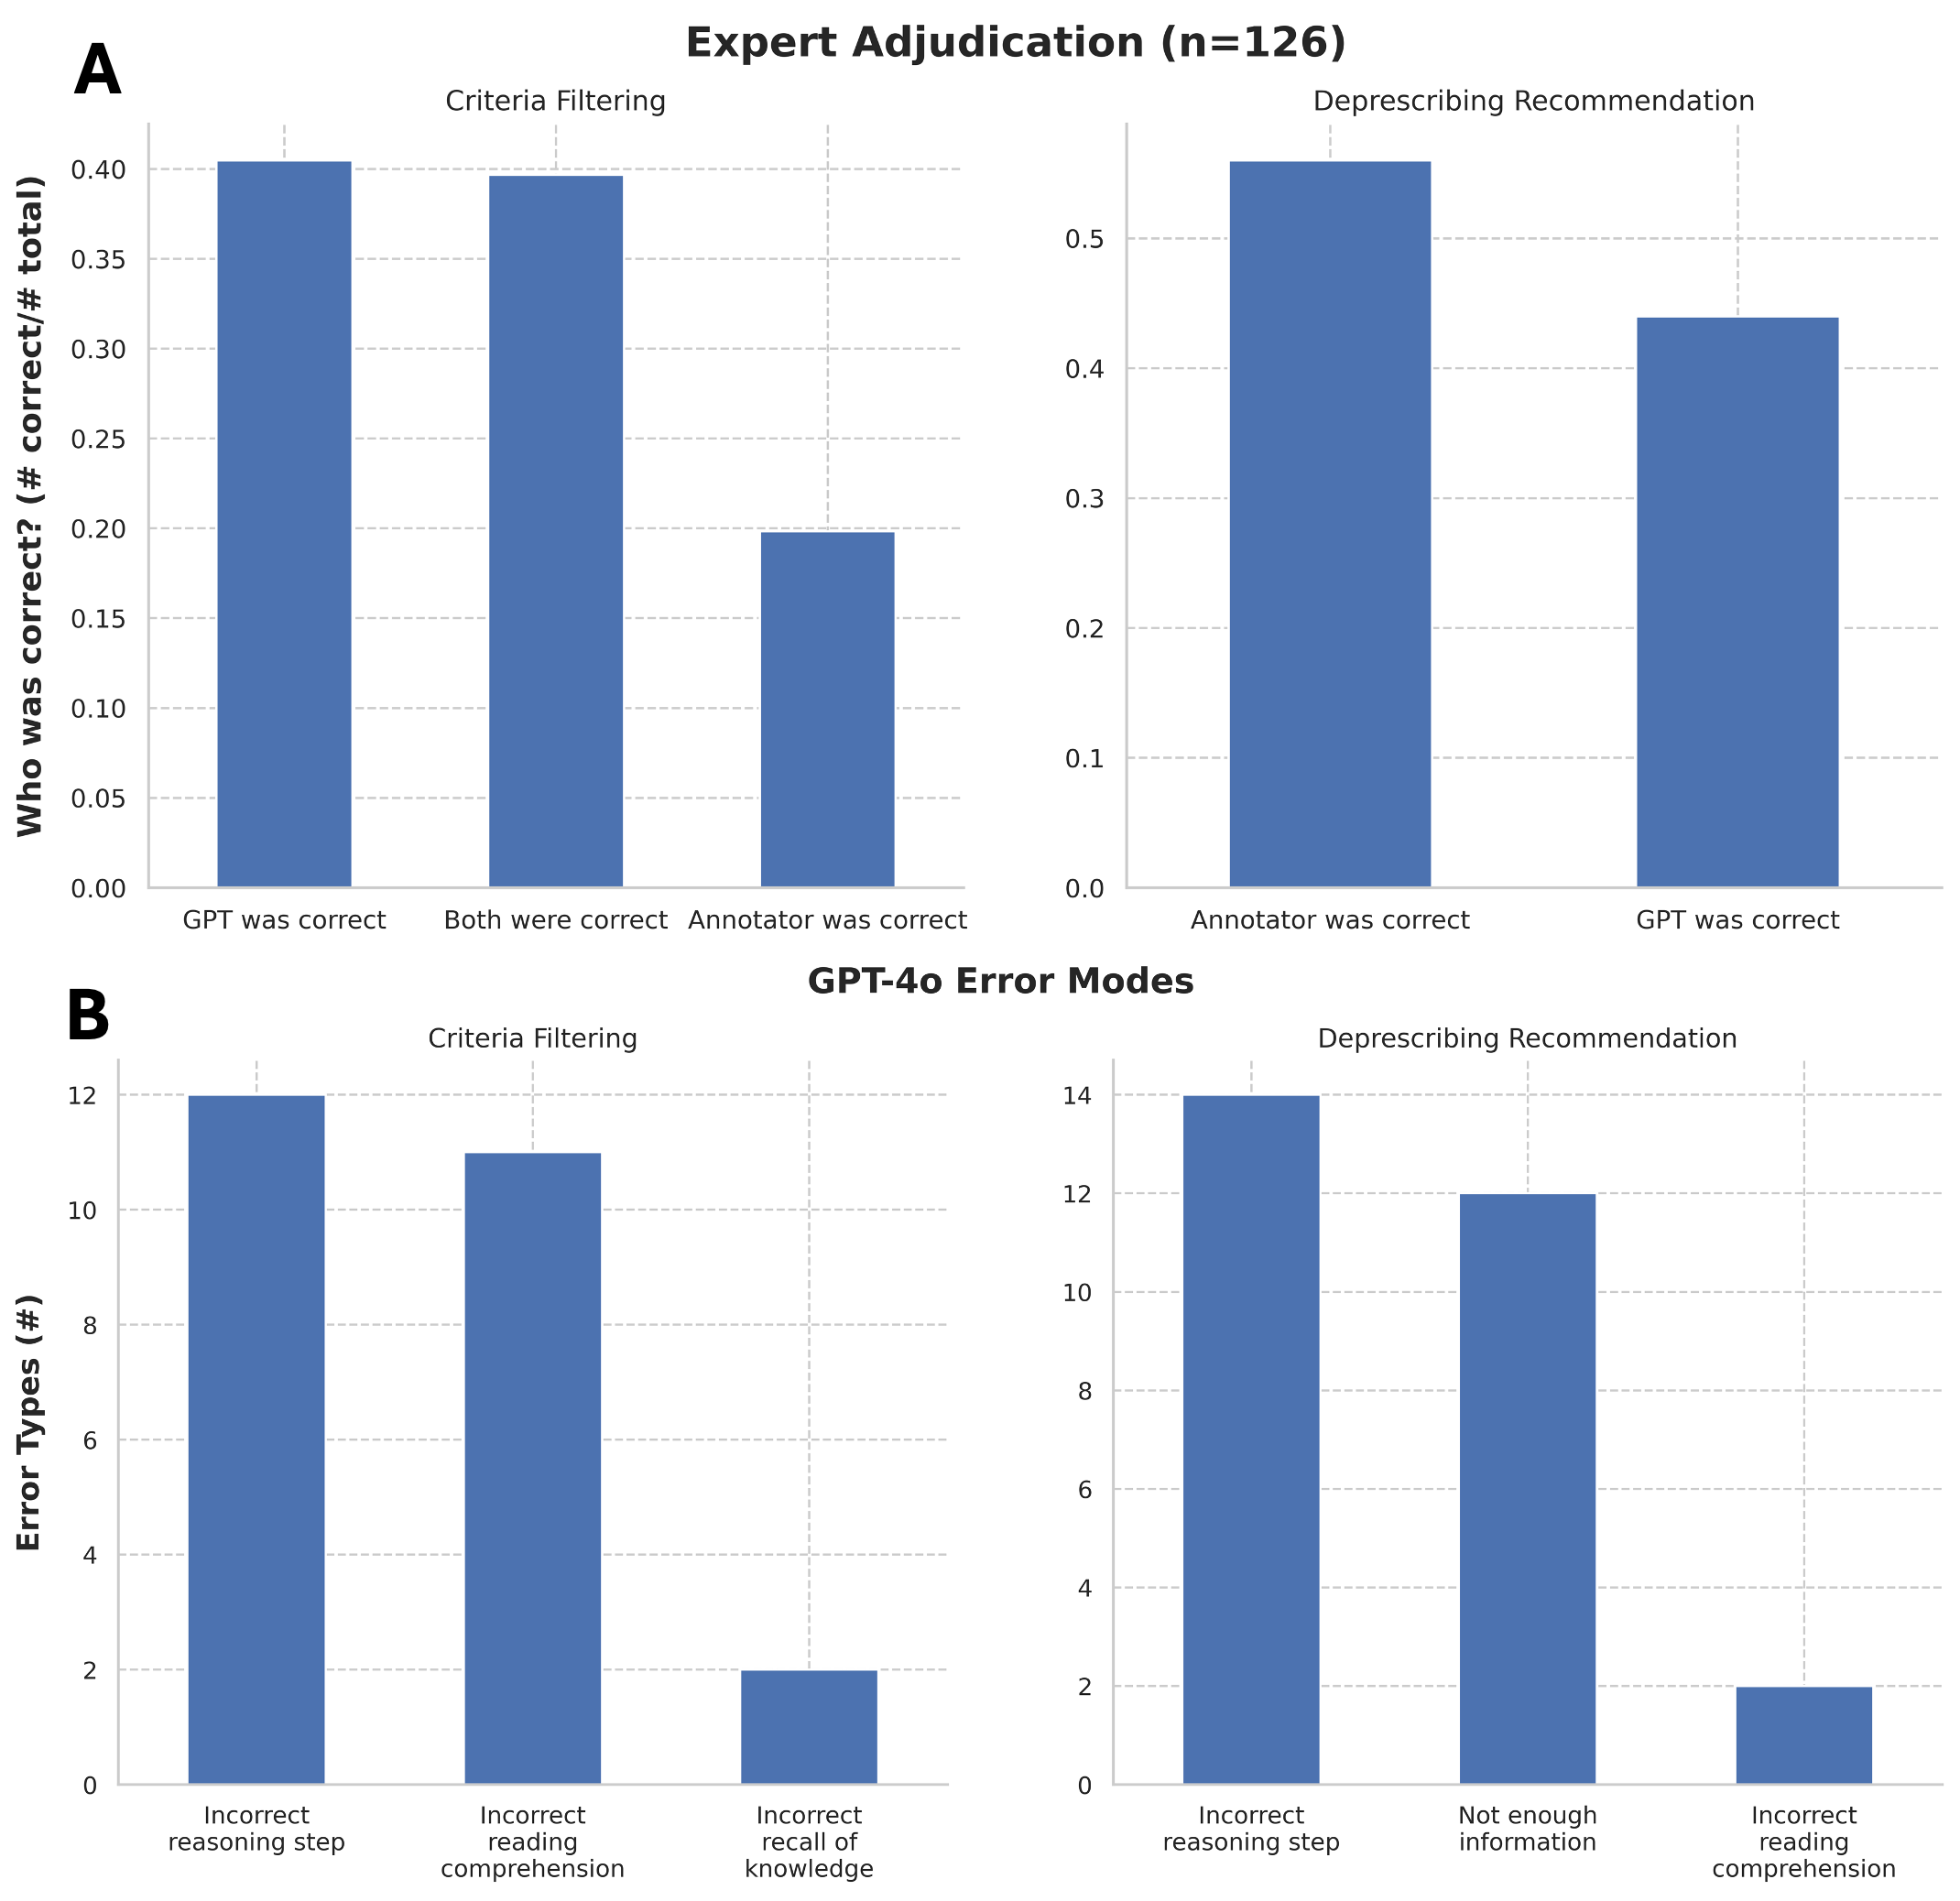
\includegraphics[width=1\textwidth] {figures/aim1/adjudication_error_types_combined.png}
	\caption{(A) Adjudication by senior clinical expert comparing junior annotators and GPT models in both criteria filtering and deprescribing recommendation tasks. (B) Types of errors by GPT-4o in the adjudication set (n=126) for both criteria filtering and deprescribing recommendation tasks.} \label{fig:aim1-error-modes}
\end{figure}


\subsection{Selective Prediction Methods}


\begin{figure}[!htbp]
	\centering
	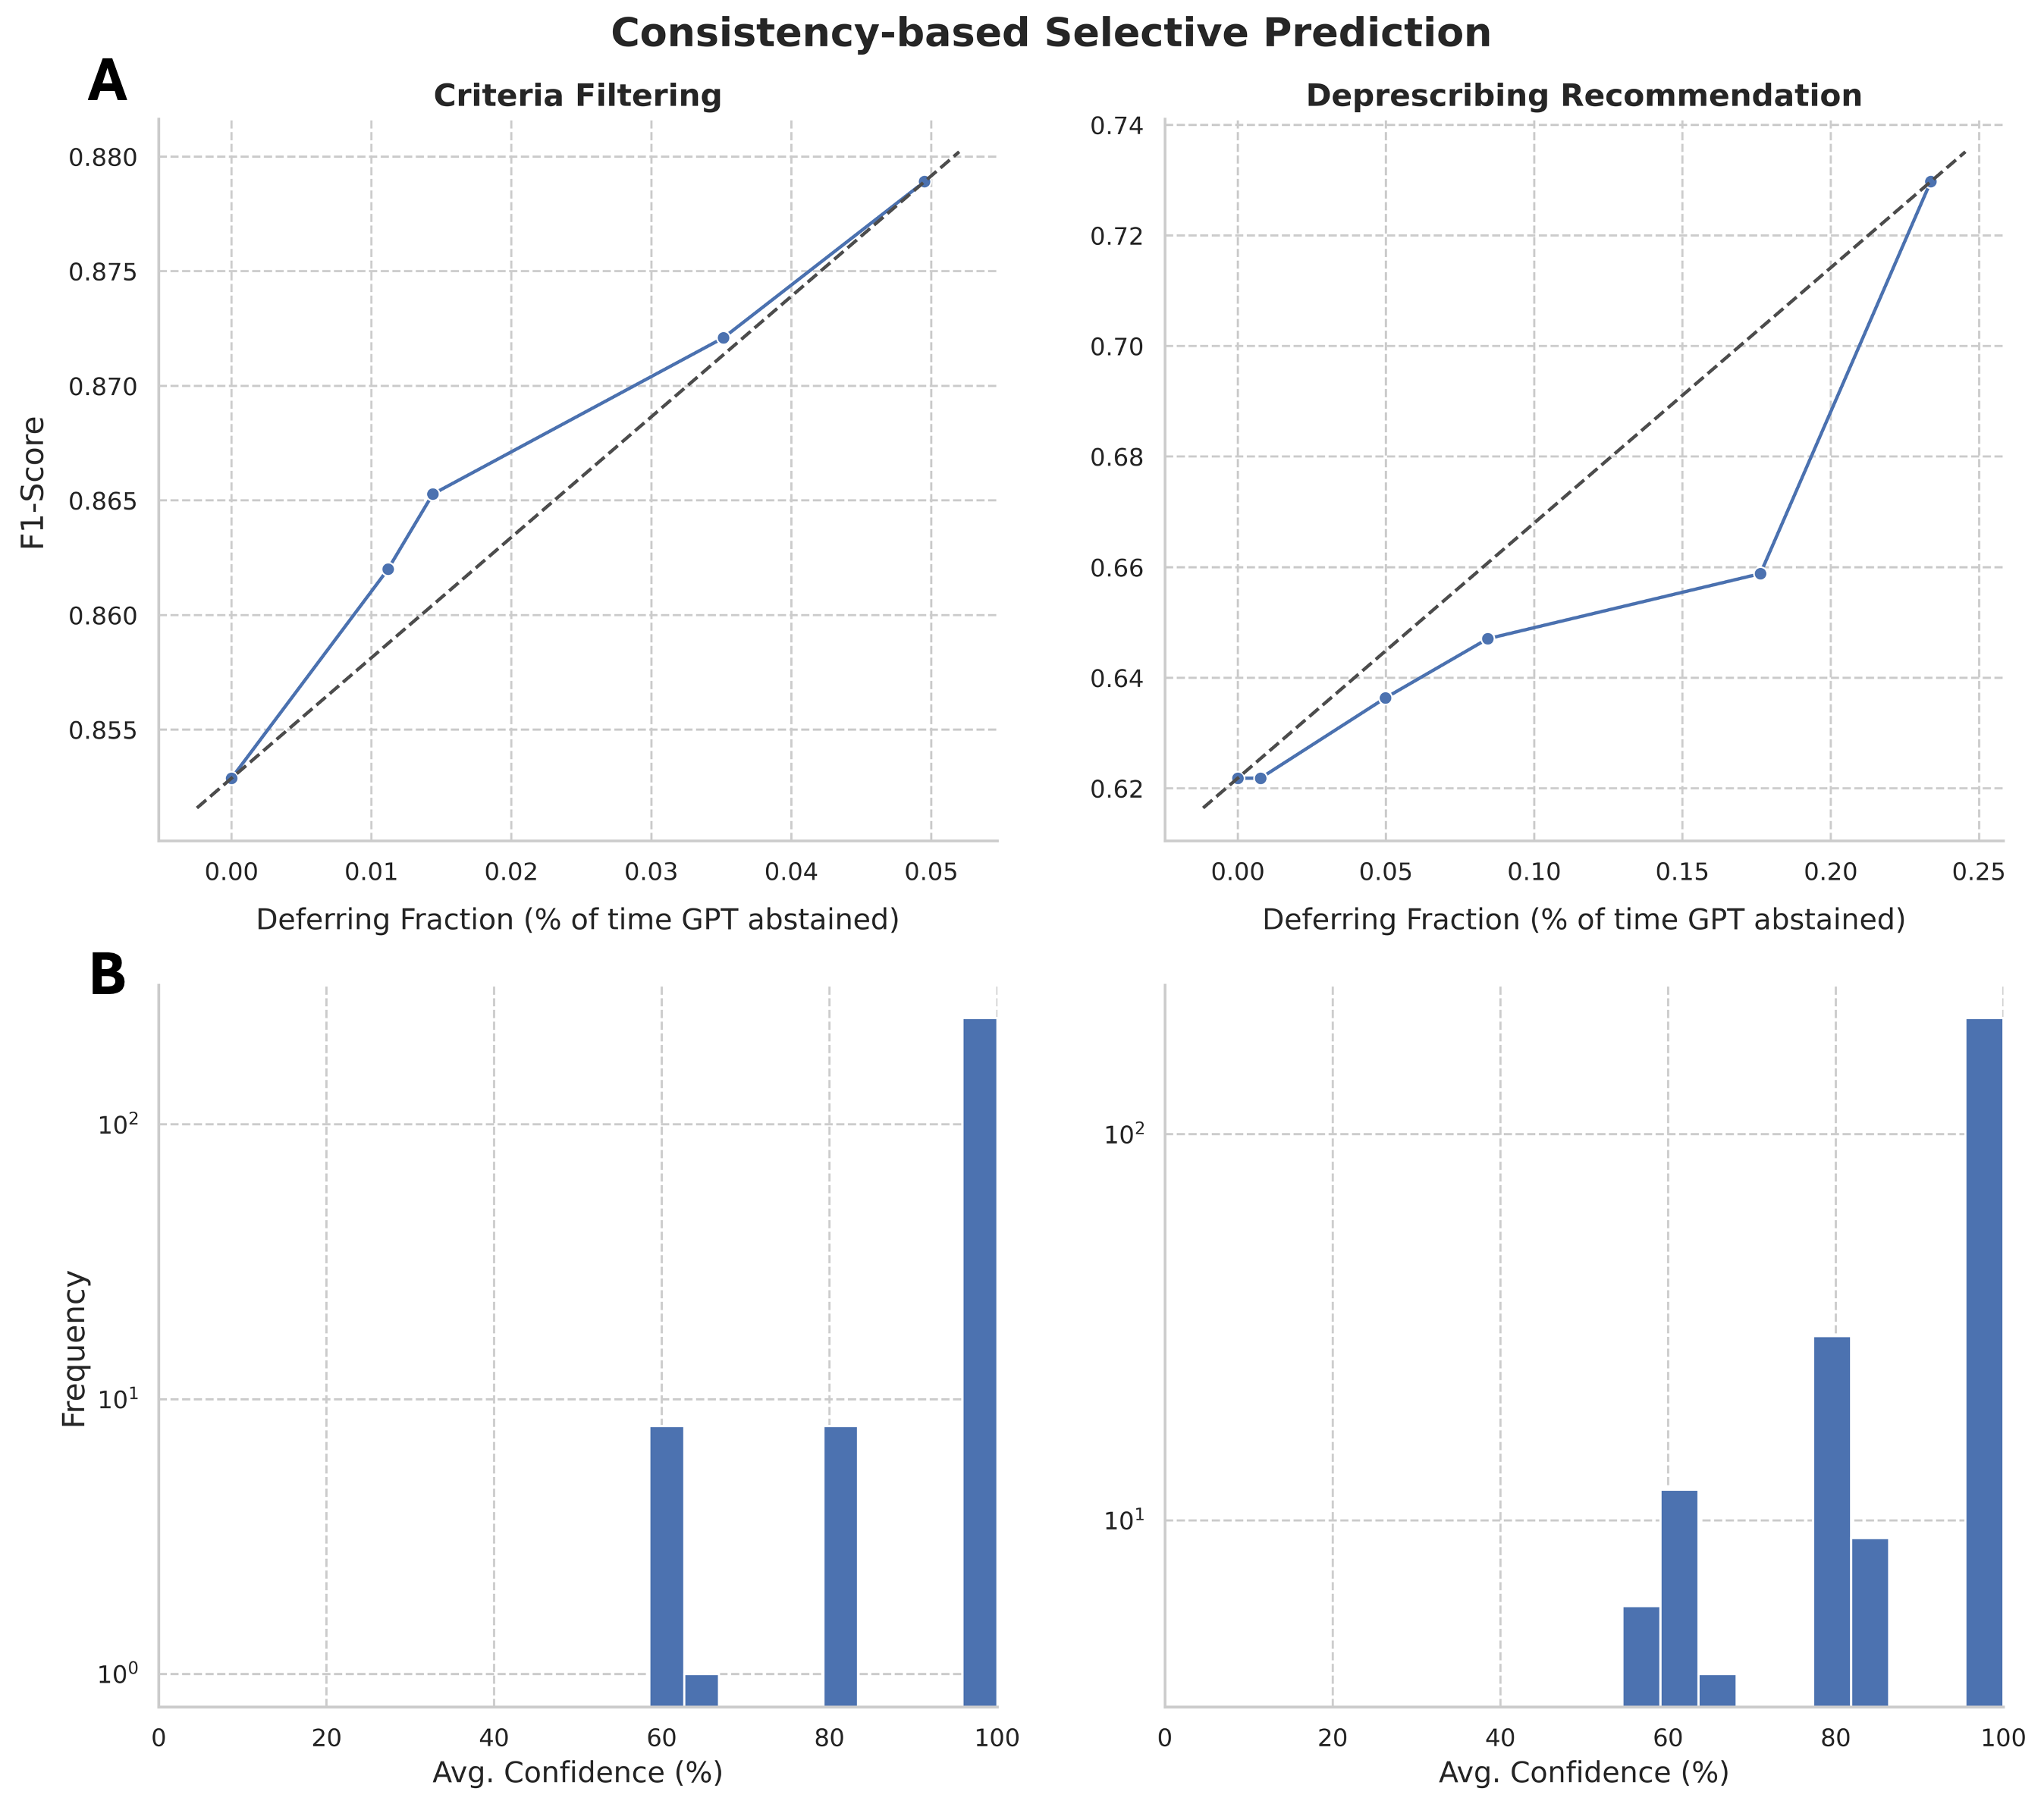
\includegraphics[width=0.8\textwidth] {figures/aim1/selective_pred_consistconf_with_dists.png}
	\caption{Joint confusion matrix across both steps showing alignment and discrepancies between GPT-4o model and medical students.} \label{fig:aim1-selective-pred}
\end{figure}


Finally, we investigated whether eliciting confidence estimates from the LLM and using them to determine if the model should abstain would improve results. We compare both verbalized confidence and consistency-based confidence to find that both forms of selective prediction improved results, albeit within a small range of F1-scores (Figure \ref{fig:aim1-verbconf} and Figure \ref{fig:aim1-selective-pred}a). In particular, consistency-based selective prediction demonstrates a positive linear relationship between accuracy in deprescribing recommendations and deferring fraction. However, despite some minor improvements, we find that the LLM is poorly calibrated, as shown in Figure \ref{fig:aim1-selective-pred}b. In general, despite consistency-based weighting, the confidence distribution is severely left-skewed with the minimum confidence being 58.5\% in eligibility filtering and 54.5\% in deprescribing recommendations. 


\section{Discussion}

In this work, we evaluated the utility of a large language model (LLM)-based pipeline, specifically GPT-4o, for identifying and recommending deprescribing opportunities for potentially inappropriate medications (PIMs) among older adults with polypharmacy in the emergency department (ED). The LLM's performance was compared to that of medical students in a two-step pipeline: filtering for criteria-eligible medications and making specific deprescribing recommendations. Adjudication by senior clinicians was used to resolve discrepancies. Finally selective prediction methods were tested to investigate the LLM's internal model of qualitative uncertainty, as well as determine how this model could be used to streamline a human-in-the-loop clinical decision making system. The results offer insights into both the capabilities and limitations of LLMs in a real-world clinical context, highlighting key areas for improvement in both LLM frameworks and deprescribing guidelines.

\subsection{Effectiveness of the Two-Step LLM Pipeline}

The LLM demonstrated strengths in the initial filtering step, accurately identifying a high proportion of medications that matched deprescribing criteria, thus offering potential to support clinicians in rapidly screening complex medication lists. In fact, the LLM outperformed medical students by a significant margin (80.1\% vs 59.5\% correct). The adjudication, combined with strong overall performance (max F1-score: 87.8\%) with a low deferring fraction, suggests that the LLM can effectively minimize the number of criteria requiring final review for deprescribing recommendations. Cases of misclassification were relatively uncommon and primarily related to nonstandard drug class names or overly broad groups, which could be improved with refined deprescribing criteria. However, in the second step—making specific deprescribing recommendations—the LLM encountered considerable difficulty, particularly when dealing with ambiguous criteria, missing information and nuanced clinical scenarios. Firstly, the LLM performed worse than the medical students, albeit by a smaller margin than in criteria filtering (56\% vs 44\% correct). In cases where the LLM produced an incorrect recommendation, this was frequently attributed to the misinterpretation of incomplete information (e.g., missing lab values), leading to false positive results. These inaccuracies may contribute to increased alert fatigue and extend the time required to interpret LLM-generated recommendations, potentially offsetting the intended efficiency gains in identifying deprescribing opportunities. This was often the case for complex inclusion/exclusion criteria that required multiple pieces of information. Our conclusions are supported by work in the clinical trial matching literature, where LLMs have demonstrated comparable performance to physicians in applying individual inclusion and exclusion criteria to identify eligible patients\citep{guptaPRISMPatientRecords2024}. One study employed a similar "filter-and-apply" pipeline, in which trials were first filtered and then matched to patients, showcasing the effectiveness of this approach\citep{ferberEndEndClinicalTrial2024}. However, despite successes in eligibility filtering, challenges remain when applying complex criteria. Similar errors to those observed in our work have been reported, such as incorrectly identifying patients who meet some, but not all, criteria, or assuming a patient with breast cancer does not have lung cancer due to a lack of explicit mention\citep{beattieUtilizingLargeLanguage2024, nievasDistillingLargeLanguage2024}. Overall, while LLMs hold promise for reducing the time burden in determining deprescribing eligibility, their application requires careful consideration, particularly in tasks involving complex reasoning.

\subsection{Role of Selective Prediction in Clinical Decision-Making}

To address the model’s limitations in clinical decision-making, we implemented selective prediction methods, which allowed the LLM to "abstain" from making a recommendation in cases of low confidence. Selective prediction marginally improved the LLM's filtering accuracy by enabling it to defer uncertain cases to human reviewers. However, the effectiveness of this approach was limited by the poorly calibrated confidence levels assigned by the LLM to its decisions. Specifically, the LLM displayed a minimum confidence level of 54\%, even in cases where its recommendations were incorrect. This indicates a tendency toward overconfidence, particularly in its deprescribing recommendations. While verbalized confidence is known to be overconfident in clinical question answering, our results contradicts recent work that suggests that consistency-based methods alleviate some of these concerns\citep{savageLargeLanguageModel2024}. This discrepancy underscores the importance of task-specific confidence thresholds and suggests that selective prediction, while useful, is not a one-size-fits-all solution in complex clinical applications. 

Although our performance was suboptimal, selective prediction methods hold promise for optimizing physician-AI workflows in real-world clinical settings. In a deprescribing CDS tool, the LLM’s confidence could be used to flag cases where the necessary information is unlikely to be inferred from available data (e.g. in the following criteria: antipsychotics at an unchanged dose for >3 months without medication review, medication reviews may not have been recorded). A well-calibrated LLM would retain human oversight while reducing the time required to initially filter medication lists, thereby allowing clinicians to focus on more complex cases where LLMs currently lack adequate reliability. Further refinement of confidence elicitation methods, tailored specifically to the nuances of clinical recommendation tasks, may enhance the model’s applicability in a broader range of clinical scenarios.

\subsection{Need for Clearer Deprescribing Guidelines}

A notable finding from this study is the need for clearer and more consistent deprescribing guidelines. Ambiguities in criteria definitions, such as those related to medication administration routes and drug classes, present substantial barriers to automation and contribute to discrepancies between human and model interpretations. For example, the requirement for “systemic” medication often lacked specification regarding inclusion or exclusion of certain administration routes, which led to frequent errors by both the LLM and adjudicators. Additionally, the model often recommended deprescribing medications that, while potentially inappropriate, required specific contextual qualifiers (e.g., patient’s life expectancy, nutritional status, frailty status) to justify deprescribing—criteria that the LLM misapplied due to lack of explicit context or ambiguous language in the guidelines. Streamlining deprescribing criteria to ensure consistent application across clinical contexts could improve model reliability and help standardize deprescribing practices. 

\subsection{Implications for LLM Use in Clinical Practice and Future Directions}

The results of this study underscore the promise of LLMs in enhancing deprescribing workflows by providing rapid filtering of PIMs, which could alleviate some of the burden on healthcare providers. However, this work also highlights the limitations of current LLMs in complex, context-sensitive clinical decision-making tasks. The LLM’s frequent tendency to over-recommend deprescribing, as compared to medical students, indicates that clear boundaries for medication eligibility and exclusion are critical for reducing false positives in automated recommendations. Cases with the potential for human harm were observed, such as suggesting deprescribing anticoagulation in a patient with recent thromboembolism. Additionally, cases were seen in which the LLM recommended deprescribing without citing a specific criteria. These behaviors suggest that strong guardrails on the LLM are needed to ensure safe, high quality recommendations. Enhancing guideline specificity, particularly for complex inclusion/exclusion criteria, could reduce both human and model error rates and may foster greater acceptance of AI-assisted deprescribing tools among clinicians. Our findings also support the potential utility of a human-in-the-loop framework, in which LLMs aid in the identification of deprescribing opportunities but defer final recommendations to clinicians. This approach not only leverages the model’s efficiency in data processing but also mitigates risks associated with erroneous recommendations, particularly in high-stakes environments like the ED. Future research should focus on refining LLM architectures to better handle the nuances of clinical reasoning and context interpretation, perhaps by incorporating more advanced natural language processing techniques and domain-specific training. Additionally, efforts to standardize deprescribing guidelines would greatly benefit the development of automated tools in this area, making them more reliable and broadly applicable.

\subsection{Limitations}

This study has several limitations that warrant consideration. First, the retrospective nature of our analysis, relying on historical data from electronic health records (EHRs), may not fully capture the complexity of real-time clinical decision-making in emergency settings. The study’s focus on a single healthcare system (Yale-New Haven Health) limits the generalizability of our findings to other settings with different patient populations, documentation patterns and healthcare practices. Second, the selective prediction methods, while providing insights into the LLM's confidence, were not universally effective, particularly in the nuanced task of deprescribing recommendations. The model’s performance in these recommendations highlights the challenge of translating structured criteria into actionable clinical decisions, especially when faced with ambiguous inclusion/exclusion conditions. Additionally, the model's reliance on textual prompts and structured EHR data may not fully account for nuanced clinical contexts that influence deprescribing decisions. Third, the small sample size for detailed analysis (100 patients) limits the statistical power and may not reflect broader patterns of medication use and deprescribing needs. Additionally, the study relied on medical students for initial annotation. While these annotations were reviewed and adjudicated by board-certified physicians, this process may introduce variability, potentially affecting the reliability of their use as a gold standard in the selective prediction methods. Lastly, the criteria used (STOPP, Beers, GEMS-Rx) were selected based on their perceived clinical risk and EHR computability, which may not encompass all relevant deprescribing scenarios. The lack of standardized guidelines for implementing deprescribing criteria in LLMs also poses a challenge for consistency and accuracy.


\section{Impact on Theory of Clinical Uncertainty}

Our initial motivation for this work was to conduct a rigorous set of evaluations on black-box LLMs to determine their ability to internalize and use clinical uncertainty in decision making in real-world clinical settings. In this work, we first explored an LLM's model of uncertainty in an ambiguous and qualitative task. This particular task was chosen, as demonstrated in the consensus evaluation, deprescribing criteria are often underspecified and ambiguous. For instance, certain inclusion/exclusion criteria required considerable clinical judgment, such as a patient's nutritional status or frailty status. Additionally, while these criteria guide recommendations for deprescribing, their implementation is often hindered by factors unrelated to the risk-benefit evaluation, such as patient expectations. For example, patients may perceive medications as a necessary treatment when visiting a provider \citep{robinsonAttitudesBarriersDeprescribing2024}, or older adults may interpret deprescribing as a sign that they are being "written off" \citep{wallisSwimmingTidePrimary2017}. These ambiguities, coupled with external factors, make the deprescribing task an ideal setting for evaluating an LLM's internal model of qualitative uncertainty and comparing it to how physicians manage such uncertainty.

The results of this experiment led to our initial theory of clinical uncertainty in LLMs. Namely, in the study, we found that an LLM was worse at recommending medications for deprescribing when compared to medical students (56\% vs 44\% correct). Moreover, when selective prediction methods were applied, LLM confidence estimation was poorly calibrated relative to its actual performance, limiting the potential benefits of these methods. Analysis of the LLM's errors revealed a pattern of unsupported reasoning, where the model made recommendations without sufficient evidence to justify them. For instance, the LLM suggested discontinuing a QT-prolonging antidepressant without history of abnormal QT intervals or a positive ECG finding. This tendency suggests that, when placed in a decision-making context requiring deprescribing recommendations, the LLM often made unsupported logical leaps to fulfill the task. Together, the findings of poor calibration and unsupported recommendations highlight how the specific context in which an LLM is tasked with decision-making can significantly influence the expression of its internal model of uncertainty and its overall performance. In the coming chapters, we discuss how our theory of the influence of clinical and role context influence and LLM's ability to estimate probabilities in a Bayesian framework and perform a conversational diagnostic task. 